% Consolidated tables matching the manuscript numbering (Tables 1--2, 5).
% Tables 3--4 appear in \texttt{results.tex} with the subsections that discuss them.

\begin{table}[p]
  \centering
  \caption{Validation results across domains.}
  \label{tab:validation}
  \small
  \scalebox{0.9}{
  \begin{tabular}{@{}llccccl@{}}
    \toprule
    \textbf{Domain} & \textbf{Tier} & \textbf{$n$ units} & \textbf{Mean $\eta$} & \textbf{SD} & \textbf{\% with $\eta>1$} & \textbf{Data source} \\
    \midrule
    Sports (Rugby)      & Primary    & \PEFrugbyNkpis  & \PEFrugbyMeanEta  & \PEFrugbySdEta  & \PEFrugbySuccess\%  & {URC} \\
    Sports (Football)   & Primary    & \PEFfootNkpis   & \PEFfootMeanEta   & \PEFfootSdEta   & \PEFfootSuccess\%   & English Championship \\
    Healthcare          & Supporting & $\PEFhealthN^{\dagger}$ & \PEFhealthMeanEta & $\PEFhealthSE^{\dagger}$ & \PEFhealthSuccess\% & \cite{nhanes2017pbxo} \\
    Clinical Genomics   & Supporting & $\PEFgenomicsN^{\ddagger}$ & \PEFgenomicsMeanEta & \PEFgenomicsSdEta & \PEFgenomicsSuccess\% & \cite{brunner2014earlybreast,geoGSE47462} \\
    Finance             & Supporting & \PEFfinanceN    & \PEFfinanceMeanEta & \PEFfinanceSdEta & \PEFfinanceSuccess\% & Yahoo Finance \\
    \bottomrule
  \end{tabular}}
  \normalsize

  \medskip
  \begin{minipage}{0.95\linewidth}\small
    \textit{Note:} Proportion with $\hat\eta>1$: share of units for which pairing reduces variance (\cref{sec:outcome_defs}). The $n$ units column counts PEF units, not participants: healthcare is one paired study of $N=10{,}352$ participants. $^{\dagger}$Paired {NHANES} oscillometric records (systolic vs diastolic, first reading); the SD column is the bootstrap standard error $\PEFhealthSE$ for the pooled $\eta$. $^{\ddagger}$Genes in the ranked subset of the {GSE47462} paired design (see Methods). That ranking prefers high $\rho$, so the percentage with $\eta>1$ is not a random-gene rate. Primary empirical tier: the sports cloud in \cref{fig:pef_landscape} and class separation against $\Delta\mathrm{ML}$ in Supplementary~\cref{fig:si_ipred_vs_dml}; the four exemplars are \cref{tab:exemplars}. Supporting tier: parameter estimation and PEF calculation summarised here and in \cref{sec:results}.
  \end{minipage}
\end{table}

\begin{table}[p]
  \centering
  \caption{Quadrant taxonomy and practical guidance.}
  \label{tab:quadrants}
  \begin{tabular}{@{}lllll@{}}
    \toprule
    \textbf{Q} & \textbf{Parameters} & $\eta$ & \textbf{What the cell records} & \textbf{Feature choice} \\
    \midrule
    Q1 & $\kappa>1$, $\rho>0$  & $>1$  & Efficient; B more variable & Not settled by the cell \\
    Q2 & $\kappa<1$, $\rho>0$  & $>1$  & Efficient; A more variable & Not settled by the cell \\
    Q3 & $\kappa<1$, $\rho<0$  & $<1$  & Inefficient; A more variable & Not settled by the cell \\
    Q4 & $\kappa>1$, $\rho<0$  & $<1$  & Inefficient; B more variable & Not settled by the cell \\
    \bottomrule
  \end{tabular}

  \medskip
  \begin{minipage}{0.95\linewidth}\small
    $\eta>1$ if and only if $\rho>0$. The $\kappa=1$ split swaps if A and B are swapped. $I(X;Y)$ is not ranked by quadrant (\cref{eq:mi_closed}). Under (A1)--(A2), $\Delta\mathrm{ML}\ge 0$. On the sports KPIs the cell does not decide the feature: the fold intervals do not separate the sign (\cref{sec:exemplars}).
    \textbf{Examples:} Q1, market-adjusted returns with A the index; Q2, the {NHANES} systolic--diastolic pair; Q3, high-volume anti-correlated sports KPIs; Q4, sports KPIs with the away side more variable and $\rho<0$.
  \end{minipage}
\end{table}

\begin{table}[p]
  \centering
  \caption{Boundary behaviour (illustrative).}
  \label{tab:boundary}
  \begin{tabular}{@{}lccc@{}}
    \toprule
    \textbf{Condition} & $\eta$ & $I(X;Y)$ & \textbf{Interpretation} \\
    \midrule
    $\kappa=1$, $\rho=0$ (Fisher) & 1.000 & 0.252 & Balanced variances, no correlation \\
    $\kappa\to 0$                 & 1.000 & 0.227 & Entity B negligible; $d_{\mathrm{rel}}\to 1$ \\
    $\kappa\to\infty$             & 1.000 & 0.279 & $d_{\mathrm{rel}}\to 0$; outcome nearest balance \\
    $\rho\to -1$ ($\kappa=1$)     & 0.500 & 0.265 & Maximum variance amplification \\
    $\rho\to +1$ ($\kappa=1$)     & $\to\infty$ & $\to 0$ & $d_{\mathrm{rel}}\to\infty$; outcome nearly certain \\
    \bottomrule
  \end{tabular}

  \medskip
  \begin{minipage}{0.95\linewidth}\small
    \textit{Note:} $I(X;Y)$ is \cref{eq:mi_closed} at $\delta/\sigma_{\mathrm{A}}=1$. As $d_{\mathrm{rel}}$ grows, $H(Y)$ falls, so the $\rho\to +1$ limit is $0$ bits rather than $1$ bit.
  \end{minipage}
\end{table}

\begin{figure}[p]
  \centering
  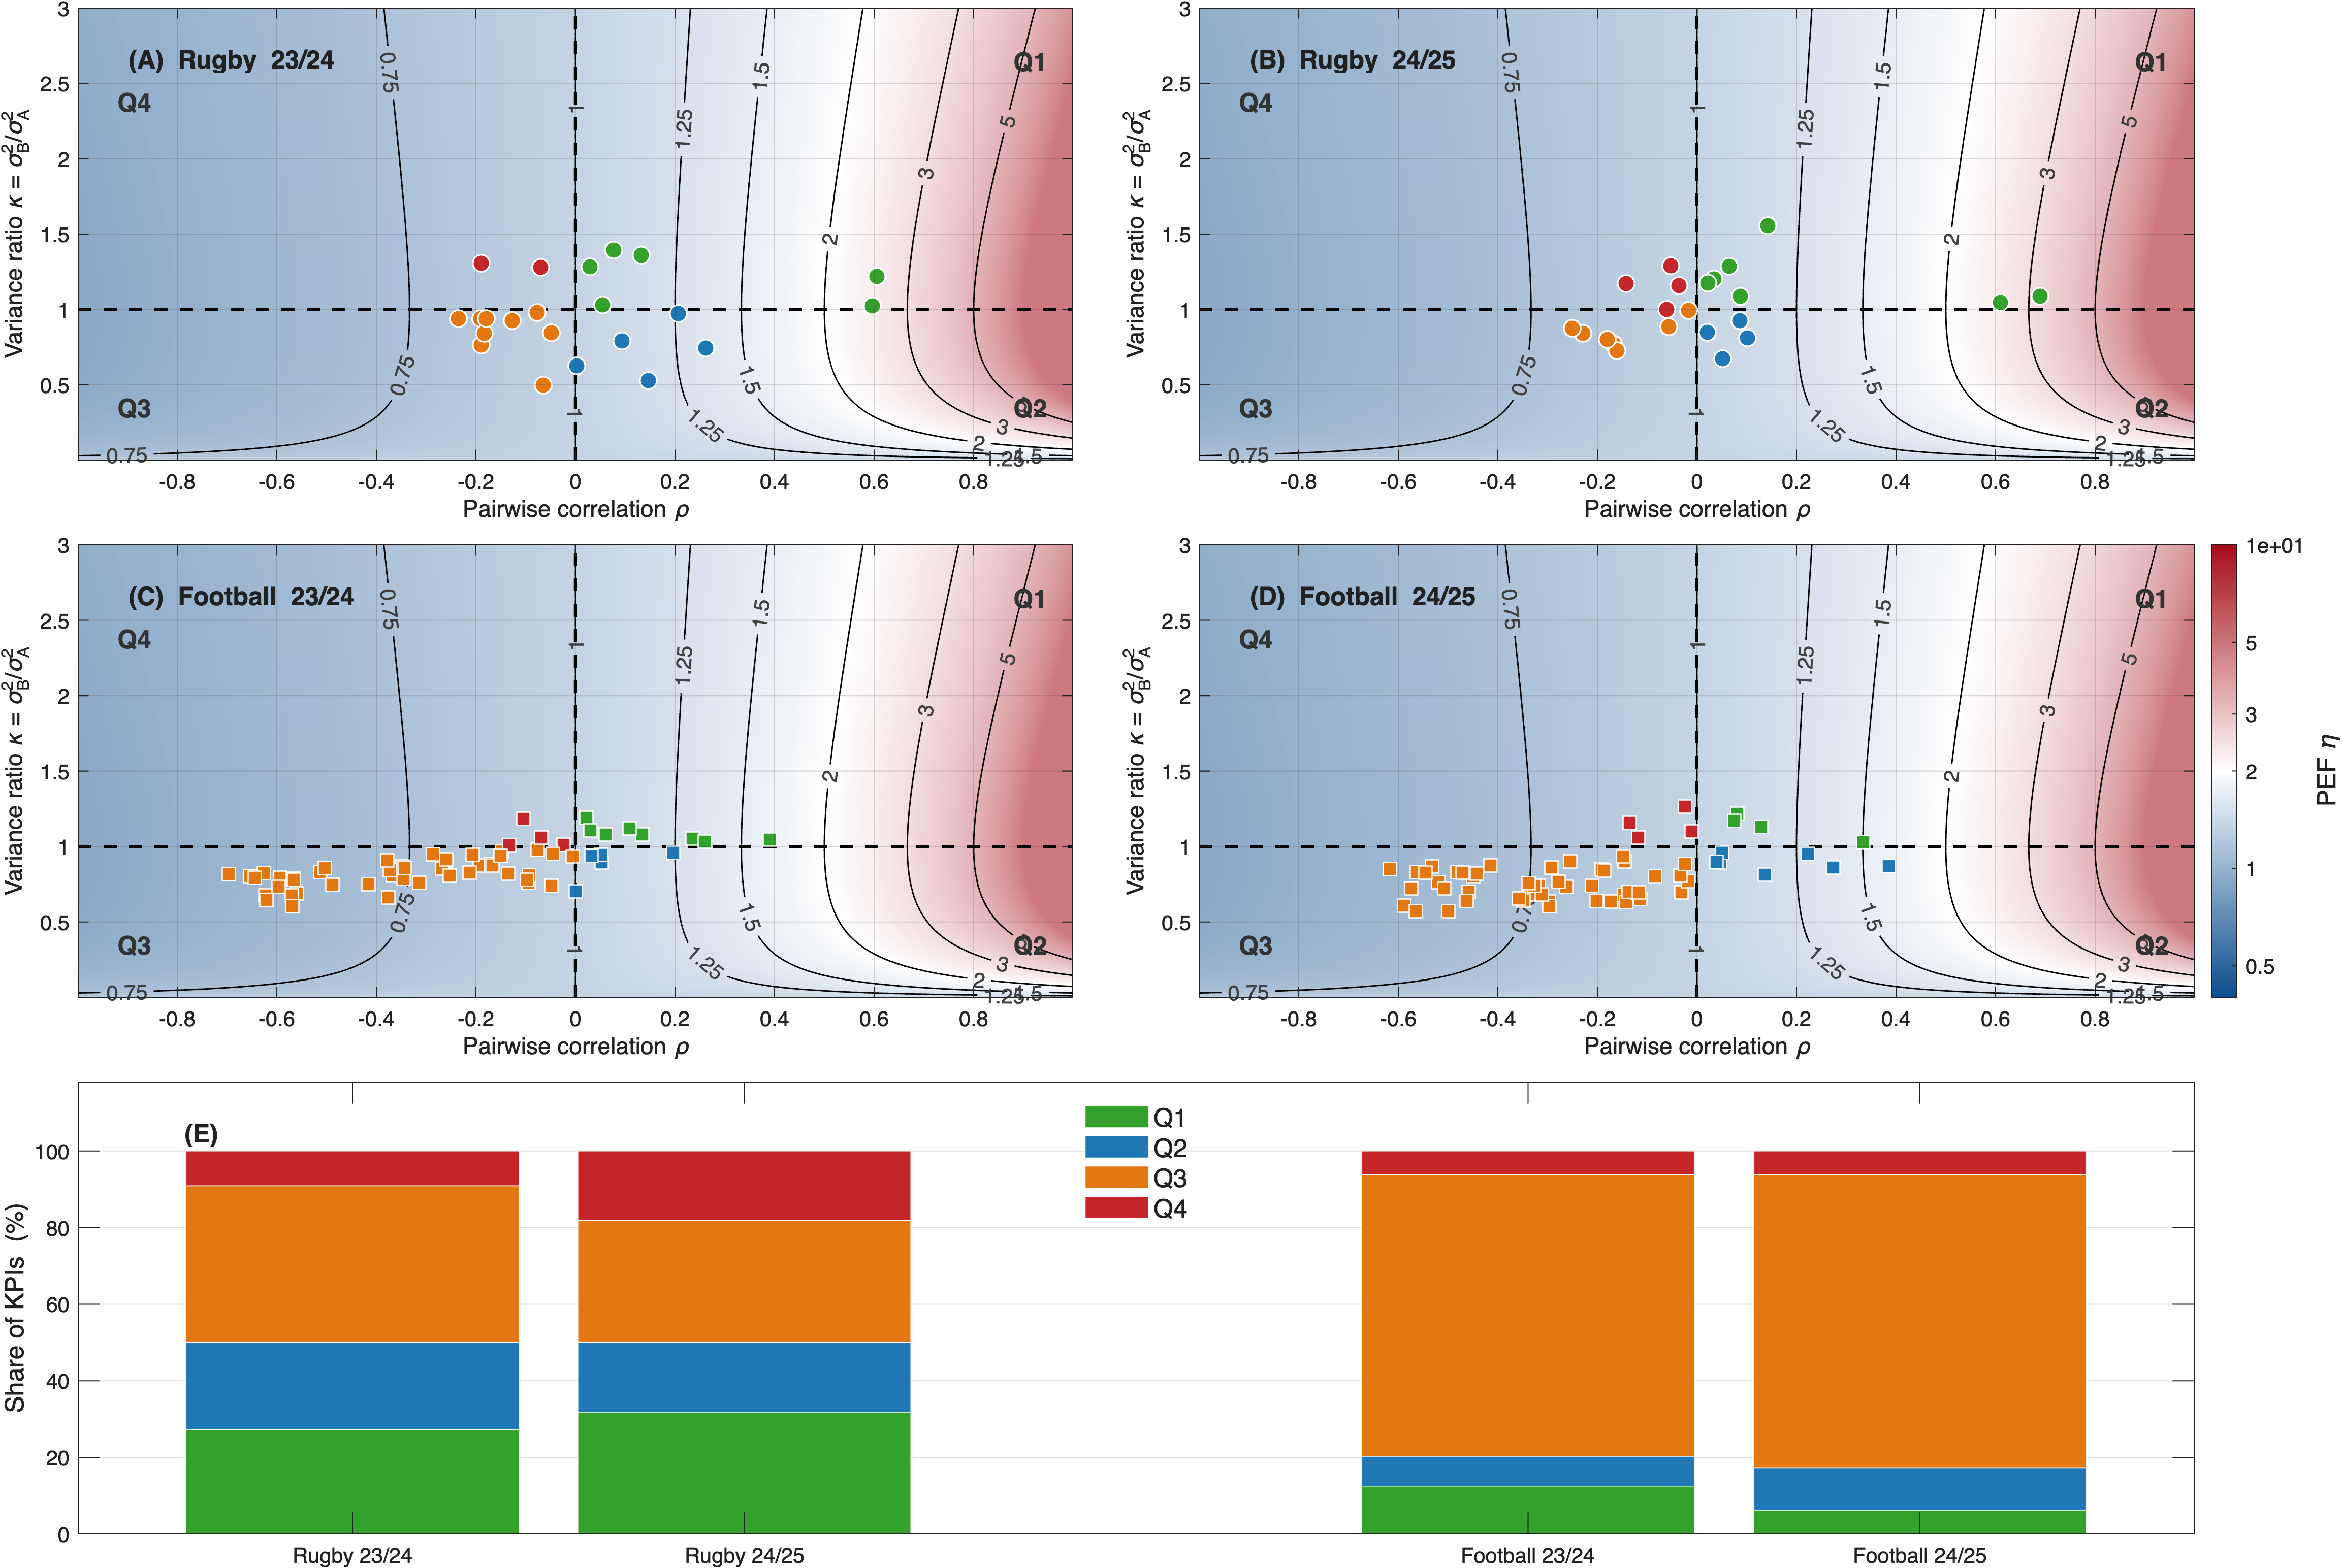
\includegraphics[width=\linewidth]{figures/Figure_S4_labelled_kpis.png}
  \caption{Sports KPI cloud on the $(\rho,\kappa)$ plane (rugby {URC}; football Championship;
    seasons 23/24--24/25). (A, B)~rugby; (C, D)~football. Markers are coloured by quadrant
    (Q1 green, Q2 blue, Q3 orange, Q4 red). (E)~share of KPIs in each quadrant, by season.
    Year-on-year identity is not traced.
    A minority of rugby KPIs cross a quadrant boundary between seasons.
    Football remains concentrated in Quadrant~3.
    The four exemplars are the rows of \cref{tab:exemplars}, not a separate panel.
    Class separation against $\Delta\mathrm{ML}$ is Supplementary~\cref{fig:si_ipred_vs_dml}.}
  \label{fig:pef_landscape}
\end{figure}

